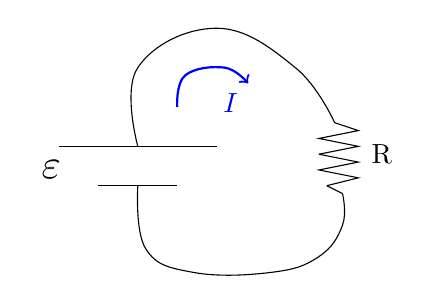
\begin{tikzpicture}
\draw (-3,1) -- (-1,1);
\draw (-2.5,0.5) -- (-1.5,0.5);
\draw  plot[smooth, tension=.7] coordinates {(-2,1) (-2,2) (-1,2.5) (0,2) (0.5,1.3)};

\draw (0.5,1.3) -- (0.8,1.2) -- (0.3,1.1) -- (0.8,1) -- (0.3,0.9);
\draw (0.3,0.9) -- (0.8,0.8) -- (0.3,0.7) -- (0.8,0.6) -- (0.4,0.5) node (v1) {};
\draw (v1.center) -- (0.6,0.4) node (v2) {};
\draw  plot[smooth, tension=.7] coordinates {(v2.center) (0.6,0) (0.3,-0.4) (-0.3,-0.6) (-1.3,-0.6) (-1.9,-0.3) (-2,0.5)};
\node at (-3.1,0.7) [scale=1.5] {$\varepsilon$};
\node at (1.1,0.9) {R};
\draw  [->, thick, blue]plot[smooth, tension=.7] coordinates {(-1.5,1.5) (-1.4,1.9) (-0.9,2) (-0.6,1.8)}node [below left]{$I$};
\end{tikzpicture}